\documentclass[aspectratio=169]{beamer}
% 默认使用hfut-sx主题,可以自由更换
\usetheme{hfut-CambridgeUS}

\usepackage{amsmath,amsfonts,amssymb}
\usepackage{multirow}
\usepackage{booktabs}
\usepackage{layout}
\usepackage{minted}
\usepackage{calligra} % 加载 calligra 字体
\usepackage[natbib=true]{biblatex}

% biblatex 数据库
\addbibresource{ref.bib}

% 幻灯片分页时从第二页开始打印“(续)”
\setbeamertemplate{frametitle continuation}[from second]

% 每一节开始的时候打印目录
\AtBeginSection[]
{
  \begin{frame}{目录}
    \tableofcontents[currentsection]
  \end{frame}
}

\newcommand{\BibTeX}{\textsc{Bib}\TeX{}}
\newcommand{\BibLaTeX}{\textsc{Bib}\LaTeX{}}
\newcommand{\Beamer}{\textsc{Beamer}}
\newcommand{\enableindent}{\setlength{\parskip}{6pt}\setlength{\parindent}{2em}}
% algorithm
\usepackage{algorithm}
\usepackage{algorithmicx,algpseudocode}
\floatname{algorithm}{算法}

\newcommand{\contactinfo}{
  \begin{center}
    Email: \href{mailto:jieyu8258@gmail.com}{jieyu8258@gmail.comemail}
  \end{center}
}


\title{本学期总结与下学期规划}
% \subtitle{副标题}
\author{王子颉}
\institute{School of Computer and Informatics, HFUT}
\date{\today}

\begin{document}

\begin{frame}
	\maketitle
	\contactinfo
\end{frame}

\begin{frame}{目录}
	\tableofcontents
\end{frame}

\section{本学期总结}

\begin{frame}
  \begin{itemize}
    \item 完成了本学期的专业课学习,成功拿到保研名额并进入了胡老师的课题组。\pause
    \item 初步的完成了毕业论文撰写,后续有更多的时间跟进课题组的工作。\pause
    \item 在保研前自学了一些实分析,泛函分析,随机过程,数值分析等数学的内容\footnote<3->{原本考虑转数学专业,但最终还是被“\textcolor{red}{学术魅魔}”胡老师吸引来了工大计算机专业,决定跟着胡老师继续在计算机专业深耕。},想从数学的角度来看待深度学习的问题。\pause
    \item 听从胡老师的建议,看完了李沐的\href{https://space.bilibili.com/1567748478/channel/seriesdetail?sid=358497}{《动手学习深度学习》}课程,看课的同时也敲了里面的一些代码,对深度学习里的一些基础网络架构有了一定了解。
  \end{itemize}
\end{frame}

\section{下学期规划}

\begin{frame}
  \begin{itemize}
    \item 补编程和数学基础,同时多看看\href{https://wbhu.net/mlapp-reading}{胡老师主页}推荐的\href{https://probml.github.io/pml-book/}{MLAPP}\footnote<1->{之前在\href{https://zhuanlan.zhihu.com/p/699377272}{知乎}上写了一些这本书的学习笔记,后续计划每周至少更新一节的内容。}等机器学习领域的好书。\pause
    \item 把一些经典的和热门的神经网络架构的文章以及胡老师发在飞书群里的文章看看,每周至少完成2-3篇。
    \begin{figure}
      \centering
      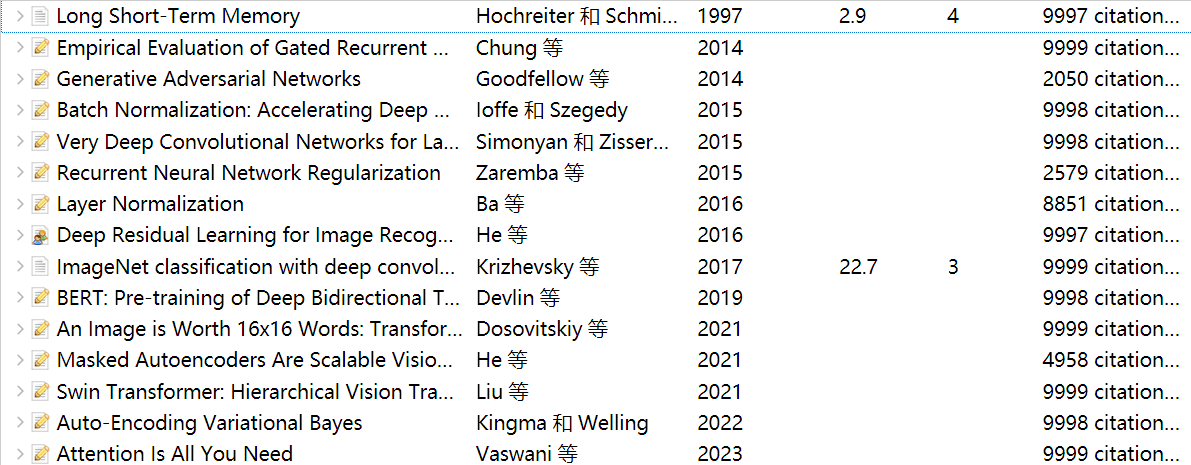
\includegraphics[width=0.6\textwidth]{images/NN.png}
    \end{figure}
    \pause
    \item 根据一篇贝叶斯深度学习\only<3->{\footcite[Position: Bayesian Deep Learning is Needed in the Age of Large-Scale AI]{papamarkou2024positionbayesiandeeplearning}}的观点类文章,精读其中提到的一些重要内容。\pause
    \item 争取在大四上结束前有小idea,并在大四下开始实验写论文。
  \end{itemize}
\end{frame}

\section{结束}
\begin{frame}[allowframebreaks]
	\frametitle{参考文献}
	{
		\tiny
		\nocite{*}
		\printbibliography[heading=none]
	}
\end{frame}

\begin{frame}
	\begin{center}
    {\Huge\calligra Thanks for your attention!}
  \end{center}
\end{frame}

\end{document}
